\documentclass[10pt]{article}

\usepackage{makeidx}
\usepackage{nopageno}

\usepackage[english]{babel}
\usepackage{blindtext}
\usepackage{graphicx, color}
\usepackage{tikz}
\DeclareGraphicsRule{*}{mps}{*}{}
\usepackage{linalgjh}
\usepackage{multirow}
\usepackage{hyperref}
\usepackage[toc]{glossaries}
\usepackage{textcomp}

\usepackage{linalgdir}

%Change the next line as appropriate for your course.
%\newcommand{\webworkurl}{http://webwork.math.ucdavis.edu/webwork2/COURSETITLE/}
\newcommand{\webworkurl}{http://webwork.math.ucdavis.edu/webwork2/LinearAlgebra/}
\newcommand{\videourl}{http://math.ucdavis.edu/~linear/videos/}

\def\nn{\nonumber}

\newtheorem{theorem}{Theorem}[section]
\newtheorem{lemma}[theorem]{Lemma}
\newtheorem{proposition}[theorem]{Proposition}
\newtheorem{corollary}[theorem]{Corollary}


\newenvironment{definition}[1][Definition]{\begin{trivlist}
\item[\hskip \labelsep {\bfseries #1}]}{\end{trivlist}}
\newenvironment{example}[1][Example]{\small \sffamily \begin{trivlist}
\item[\hskip \labelsep {\bfseries #1}]}{\end{trivlist}}
\newenvironment{remark}[1][Remark]{\begin{trivlist}
\item[\hskip \labelsep {\bfseries #1}]}{\end{trivlist}}

\DeclareMathOperator{\tr}{tr}
\DeclareMathOperator{\rref}{RREF}

% sideremark
\def\sideremark#1{\ifvmode\leavevmode\fi\vadjust{\vbox to0pt{\vss
\hbox to 0pt{\hskip\hsize\hskip1em
\vbox{\hsize3cm\tiny\raggedright\pretolerance10000
 \noindent #1\hfill}\hss}\vbox to8pt{\vfil}\vss}}}


\newcommand{\edz}[1]{\sideremark{#1}}
\def\idx#1{{\em #1\/}} % ****

\newcommand{\1}{{\rm 1\hspace*{-0.4ex}%
\rule{0.1ex}{1.52ex}\hspace*{0.2ex}}}

\DeclareMathOperator{\cofactor}{cofactor}
\DeclareMathOperator{\spa}{span}
\DeclareMathOperator{\nul}{null}

%%Undoes phoney newpages
\newcommand{\phantomnewpage}{\newpage}

\makeindex

\makeglossaries


%------------------------------------------------
% TODO LIST
% 0) We moved sections 17,18,19 and 24.
% 1) Reorder WebWork to match section reordering.
% 2) Read through, check for dependency problems.
% 3) Fu's list of corrections
% 4) notes2: Worked example with no solutions
% 
% 
% 
\newcommand{\inputProblems}[1]{\section*{Review Problems} \input{#1}}

\oddsidemargin -10mm
\evensidemargin 3mm
\topmargin -10mm
\headheight 0mm
\headsep 0mm
\textheight 220mm
\textwidth 185mm
\footskip 8mm


% This command works by specifying the following (in order):
%  1 - the filename (with extension)
%  2 - the text describing the video
%  3 - The hyperlink reference
% For example we have
% \videoscriptlink{gaussian_elimination_more_background.mp4}{Augmented Matrix Notation~\ref{ge4} and~\ref{ge5}}{script_gaussian_elimination_more}
\newcommand{\videoscriptlink}[3]{
\begin{center}
\href{\videourl #1}{\raisebox{-.4cm}{
\includegraphics[scale=.075]{take1.jpg}}} \hspace{1cm}\scalebox{1.2}{\tt #2}
\hspace{1cm} {\raisebox{-.3cm}{
\includegraphics[scale=.08]{script.jpg}}}
\end{center}
} % videoscriptlink definition


%\newcommand{\probleminput}[2]{\section{#1} \input{#2}}

\newcommand{\problemtitle}[1]{\section{Problems: #1}}
\newcommand{\probleminput}[1]{\input{#1}}

\begin{document}

\pagestyle{plain}

\title{Problem Sets for Linear Algebra in Twenty Five Lectures}




\maketitle

\begin{center}
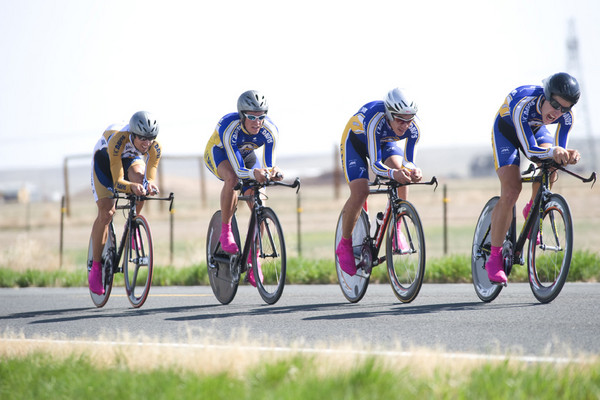
\includegraphics[scale=.6]{bikes.jpg}\\[8mm]
\end{center}

\begin{center}
Selected  problems for students to hand in.
\end{center}

\newpage

\tableofcontents

\newpage

\problemtitle{\whatIsTitle}
\probleminput{\whatIsPath/problems}

\problemtitle{\gaussElimTitle}
\probleminput{\gaussElimPath/problems}

\problemtitle{\elemRowOpsTitle}
\probleminput{\elemRowOpsPath/problems}

\problemtitle{\solutionSetsTitle}
\probleminput{\solutionSetsPath/problems}

\problemtitle{\vectorsInSpaceTitle}
\probleminput{\vectorsInSpacePath/problems}

\problemtitle{\vectorSpacesTitle}
\probleminput{\vectorSpacesPath/problems}

\problemtitle{\linTransTitle}
\probleminput{\linTransPath/problems}


\problemtitle{\matricesTitle}
\probleminput{\matricesPath/problems}

\problemtitle{\propMatricesTitle}
\probleminput{\propMatricesPath/problems}

\problemtitle{\inverseMatTitle}
\probleminput{\inverseMatPath/problems}

\problemtitle{\luDecompTitle}
\probleminput{\luDecompPath/problems}

\problemtitle{\elemMatDetTitle}
\probleminput{\elemMatDetPath/problems}

\problemtitle{\elemMatDetIITitle}
\probleminput{\elemMatDetIIPath/problems}

\problemtitle{\propDetTitle}
\probleminput{\propDetPath/problems}

\problemtitle{\subspacesTitle}
\probleminput{\subspacesPath/problems}

\problemtitle{\linIndepTitle}
\probleminput{\linIndepPath/problems}

\problemtitle{\basisDimTitle}
\probleminput{\basisDimPath/problems}

\problemtitle{\eigenTitle}
\probleminput{\eigenPath/problems}

\problemtitle{\eigenIITitle}
\probleminput{\eigenIIPath/problems}

\problemtitle{\diagTitle}
\probleminput{\diagPath/problems}

\problemtitle{\orthonormTitle}
\probleminput{\orthonormPath/problems}

\problemtitle{\gramSchmidtTitle}
\probleminput{\gramSchmidtPath/problems}

\problemtitle{\diagSymMatTitle}
\probleminput{\diagSymMatPath/problems}

\problemtitle{\kernelTitle}
\probleminput{\kernelPath/problems}

\problemtitle{\leastSquaresTitle}
\probleminput{\leastSquaresPath/problems}

\end{document}





\end{document}
